\chapter{Middle-level Intermediate Representation}

This chapter describes SableWasm's middle-level intermediate representation
(MIR), which has a critical role in the entire compilation pipeline. The MIR
acts as a middle ground between the WebAssembly bytecode frontend and various
possible backends. Currently SableWasm only implements one backend that utilizes
the LLVM compilation framework, but adding more backend support should not
require significant modification on the MIR. It also implements an analysis and
transformation framework where we perform several optimizations over the MIR. We
will first go over the overall design of the MIR, then later move to the
translation strategy we used to translate WebAssembly bytecode to MIR. Finally,
we will end the chapter with several analyses and transformations we
implemented.

\section{MIR Design}

In the previous chapters, we covered the design of WebAssembly bytecode. A quick
reminder, WebAssembly is a stack-based intermediate representation (IR) where
all instructions operate over an implicitly declared operand stack. There are
several advantages of a stack-based IR. Perhaps the most important one is its
portability. A stack-based IR makes fewer assumptions on the machine than a
register-based one. One can even provide an implementation for a hypothetical
machine with only one register. Another advantage is the code size. Experiments
show that, in general, a stack-based IR is smaller in size than its
corresponding registered version \cite{stack-and-register-vm}. When designing a
binary format that ships executables over the internet, the stack-based IR seems
to be a better choice for WebAssembly.

Nevertheless, there are no silver bullets: a stack-based IR design also has its
drawbacks. One of them is the difficulty faced when performing code analysis and
transformation over the module. As for each instruction, its operands implicitly
come from the stack; the value use-definition relationship between instructions
is not apparent to the analysis, and recovering such connection between
instructions from the IR is not a trivial task.

\begin{figure}
    \centering
    \lstinputlisting[
        language=SableWasmMIR,
        basicstyle=\linespread{0.8}\ttfamily,
        numbers=left
    ]{Code/4.MIR/fibonacci.mir}
    \caption{Fibonacci in translated SableWasm MIR}
    \label{fig:mir-fibonacci}
\end{figure}

On the other hand, we have the register-based intermediate representation,
commonly abstracted to assume an infinite number of registers and requiring a
register allocation algorithm to map them to actual, physical registers. For
each instruction in register-based IR, it has its operand encoded in the
instruction. Hence, the use-definition relationship will become explicit to the
analysis and transformation.

The main design goal for SableWasm MIR is to provide an analysis platform for
the entire compiler system. Thus, we implement our MIR as an infinite register
machine. We also take a traditional approach in various other aspects. For
example, instead of using the structured control flow similar to what
WebAssembly offers, we use \emph{control-flow graphs} (CFGs) to represent the
relationship between basic blocks. The SableWasm MIR is also in
\emph{single static assignment} (SSA) form \cite{ibm-ssa}, as covered in the
background chapter. The design for instruction and module-level entities in
SableWasm MIR is quite similar to what WebAssembly instruction offers. One can
view the SableWasm MIR as a mixture of the target LLVM intermediate
representation and the source WebAssembly bytecode. We also adopt several design
features from LLVM IR into MIR, such as automatically managed use-site lists,
which provide each AST node with an efficient way to access their use sites.
In SableWasm MIR, all elements are derived from the base class \texttt{ASTNode}
which implements these features that are helpful later in MIR analysis and
transformation.

Figure~\ref{fig:mir-fibonacci} shows a simple function that calculates Fibonacci
numbers with a recursive method in SableWasm MIR. With the help of the figure,
we will go through the detailed design of SableWasm later in the chapter. We
will first present the module-level entity design and their initializer
expressions, such as functions, then move to the design of each instruction
defined in MIR.

\section{MIR Module Entities}
\label{section:mir-design-module-entities}

\begin{figure}
  \centering
  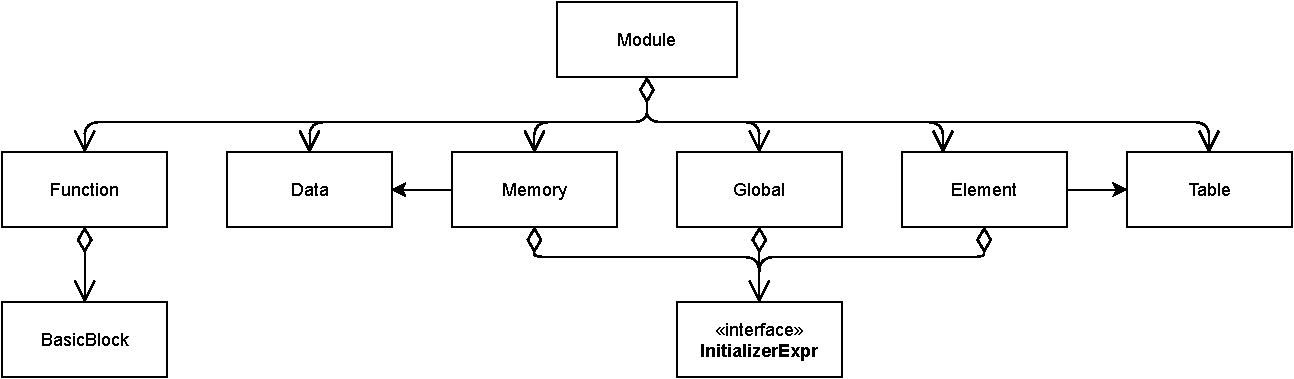
\includegraphics[width=\textwidth]{Images/4.MIR/module.pdf}
  \caption{SableWasm MIR Module-level entities}
  \label{fig:sablewasm-mir-module}
\end{figure}

SableWasm module-level entities are the top-level elements in a translation
module. They are direct implementations of the WebAssembly module entities
defined in the specification. Figure~\ref{fig:sablewasm-mir-module} presents a
general illustration of the SableWasm module-level entities. In this section,
we will cover the design of each entity and compare it with its WebAssembly
correspondent. All SableWasm module-level entities can optionally have import
and export annotates, except \texttt{data} and \texttt{element}. These
annotations correspond to the import and export entries defined in the
WebAssembly specification.

\paragraph{Function}
In figure~\ref{fig:mir-fibonacci}, we have a function definition at line 8. A
function declaration in SableWasm provides information about the type, local
variables, and name. A function definition should satisfy all the function
declaration requirements and, in addition, provide a function body using basic
blocks. The design of the function declaration and definition in SableWasm is
quite similar to that of WebAssembly. The only major difference is how to
represent the function body. We will come back to this in the later sections
within this chapter when we discuses the design of SableWasm MIR instructions.

\paragraph{Global}
SableWasm's global variable declaration and definition follow the design in
WebAssembly. In SableWasm, we relax several of the constraints defined in the
WebAssembly specification and its extensions. In the SIMD extension proposal,
the 128-bit vector type, \texttt{v128}, is only suitable within the function
body. There is no direct way to pass a vector value to the host environment, as
there is a lack of standard representation for 128-bit packed vectors in
JavaScript \footnote{This might subject to change in the future.}. In SableWasm,
we treat all primitive types uniformly. Thus, a global variable can contain an
integral value, a floating-point value, or even a packed SIMD vector. The type
for the SableWasm MIR global variable follows the specification in WebAssembly;
it consists of a value type and a constness modifier. In
figure~\ref{fig:mir-fibonacci}, we have a global variable definition at line 6,
which introduces a mutable 32-bit integral value. All global variable
definitions in SableWasm must provide a value initialization via an initializer
expression. In SableWasm MIR, all initialization expressions are constant
expressions, meaning that the host system can deduce the resulting values at the
module initialization phase. At runtime, the host system will first evaluate
these expressions and then initialize the global variables accordingly.
We will come back to the initialization expressions in detail later in this
chapter.

\paragraph{Memory and Data}
Memory and Data are implementations of the WebAssembly linear memory and its
initializer, respectively. One might think that there is no need to separate the
memory initializer from the memory entity definition, as in WebAssembly
specification, all data section entries must provide a valid linear memory
index. In the early version of SableWasm, we indeed adopt such implementation.
However, this approach might be subject to a significant change in an extension
that might soon merge to the WebAssembly specification. The WebAssembly bulk
memory operation extension proposal \footnote{WebAssembly bulk memory
  operations: \\\url{https://github.com/WebAssembly/bulk-memory-operations}}
introduces new instructions, such as \texttt{memory.fill} that directly refers
to a data section segment. Moreover, the proposal relaxes the constraints on the
linear memory index. Now the index can behave as a flag indicating whether the
data segment itself is active or not and no longer serves as a linear memory
index. Hence, to make our framework `futureproof', we separate linear memory
declarations from their initializers. Figure~\ref{fig:mir-fibonacci} presents a
linear memory definition at line 2. SableWasm memory entities also adopt
WebAssembly's linear memory type. The type consists of a pair of unsigned
integers, indicating the lower bound and upper bound of the memory size in
WebAssembly pages. The example above defines a memory with a minimal size of 2
pages, 128KiB, and exports it under the name `memory'. It, however, does not
provide any example for data initializers, although they are quite easy to
understand: a data initializer is essentially a binary chunk with an
initialization offset, and is semantically equivalent to a data section entry
in an ELF file.

\paragraph{Table and Element}
SableWasm's table and element entity implement the indirect table and its
initializer, namely element segment, accordingly. They follow the same principle
as the memory and data entity in the previous section. Currently, like a data
segment entry, WebAssembly's element section entry must refer to a valid
indirect table via an index. In the future, this may also subject to change. The
WebAssembly reference types extension proposal \footnote{WebAssembly reference
  types: \url{https://github.com/WebAssembly/reference-types}} introduces
instructions such as \texttt{table.fill} that are able to have direct access to
element segment initializers. \texttt{table.fill} instruction is similar to
\texttt{memory.fill} defined in the bulk memory operation extension. It will
copy a sequence of compile-time defined function pointers into an indirect table
at runtime. Thus, when we design our table entity, we also split the
declarations from their initializers. The type for table entity is the same as
the table type in WebAssembly. It consists of a pair of unsigned integers,
indicating the lower bound and upper bound for the number of function pointers
stored in the indirect table. In SableWasm MIR, we treat memory entities and
table entities as black boxes, and its concrete implementation is deferred to
the backend. In the example shown in figure~\ref{fig:mir-fibonacci}, the module
defines a table entity at line 4 that stores exactly one function pointer. Note
that the table entity does not require users to initialize the value for all
entries. The table entity default initializes all entries to null pointers.

In this section, we covered the design for module-level entities in SableWasm.
They are pretty similar to the those defined in the WebAssembly specification.
In the next section, we will move the design of SableWasm initialization
expressions.
\subsection{MIR Initializer Expressions}

\begin{figure}
  \centering
  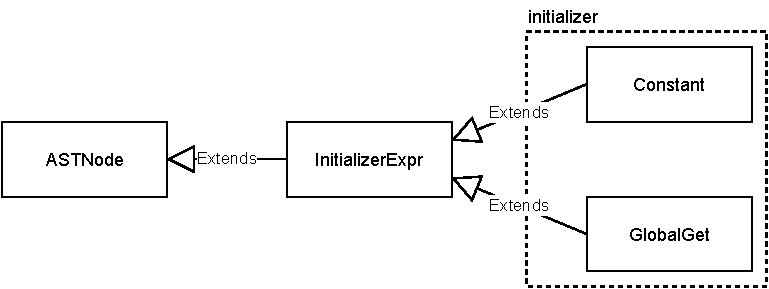
\includegraphics[width=0.85\textwidth]{Images/4.MIR/initalizer-expression.pdf}
  \caption{SableWasm MIR Initializer Expression}
  \label{fig:sablewasm-mir-initializer-expression}
\end{figure}

WebAssembly defines a particular form of expression for initialization, namely
constant expressions. They can appear in three locations in the current
specification. First, global variables declaration can contain constant
expression as their initialization values. Additionally, data section entries
and element section entries can have constant expressions as the offsets for
their initialization payload. In SableWasm MIR, we define initializer
expressions that act similar to what constant expressions do in WebAssembly.
Figure~\ref{fig:sablewasm-mir-initializer-expression} gives a general
illustration about SableWasm MIR initializer expressions. The initializer
expressions are quite simple. In the current WebAssembly and SableWasm, an
initializer expression can be either a constant value or refer to an imported
global via \texttt{GlobalGet} instruction. Hence, in principle, currently,
a SableWasm MIR initializer expression is essentially a single instruction. In
the future, one may generalize such constraints by allowing more complex
constructs in initializer expressions.

\paragraph{Constant}
The \texttt{Constant} instruction represents a single constant value for the
initializer expression. In WebAssembly, a constant value can be one of the
following: a 32-bit or 64-bit integer, a floating-pointer number, or a 128-bit
SIMD vector \footnote{With WebAssembly SIMD128 extension}, and the specification
encodes the type within the instruction opcode. Hence, there are multiple
instructions in WebAssembly to introduce a constant. In SableWasm, we do not
encode the type into the opcode, and \texttt{Constant} instruction is the only
instruction that takes care of the task. In figure~\ref{fig:mir-fibonacci}, we
have a constant initializer at line 6 that initializes the value of the global
to a 32-bit integer with a value that equals 66560. When querying the type of a
\texttt{Constant} instruction, SableWasm will infer it according to its payload
constant.

\paragraph{GlobalGet}
The \texttt{GlobalGet} instruction is exactly same as the WebAssembly's
\texttt{global.get} in terms of execution semantics. The WebAssembly
specification allows any initializer expression to refer to an imported
\footnote{This might subject to change in the future version of WebAssembly}
global value. As these values are initialized before entering the module,
reading their value is always valid during module initialization. The example
in figure~\ref{fig:mir-fibonacci} does not provide an example of
\texttt{GlobalGet} as an initializer expression, as they are less frequently
used compared to constant initializer expression, especially for global values.
However, in some ABI implementations, data section entries and element section
entries require reading from global values serving as base pointers. SableWasm
also infer the type for \texttt{GlobalGet} initializer expression in a similar
fashion as \texttt{Constant}. In this case, the type of instruction is the same
as the referred global variable without the `constant' modifier.

In this section, we covered the design and implementation of initializer
expressions in SableWasm. They are pretty simple in the current design. We will
now move to the next part in the SableWasm design, the MIR instructions.
\section{MIR Instructions}

SableWasm MIR uses a control-flow-graph (CFG) based representation in
\emph{static single assignment} (SSA) form to represent code body in function
definitions. We have provided an introduction to CFG and SSA in the background
chapter. Here is a quick recap. CFG splits the control flow within the function
into basic blocks. A basic block represents the most extended instruction
sequence without control flow transfer, such as branching. Note that for
function calls, we take a similar approach to that of LLVM. We will come back
to this in detail later in this section. Additionally, SSA requires that all
values must have unique definition sites. Hence, in SSA form, the
use-definition chain is trivial to compute, while in a traditional CFG, one
would need to extract this from the graph with the help of a \emph{reaching
  definition} analysis. The SableWasm MIR instruction set is similar to
WebAssembly bytecode in terms of semantics for most of the instructions.
However, it operates over an infinite register machine instead of a
stack-based machine, and in some cases, semantics differ in order to keep the
size of the SableWasm instruction minimal. In this section, we will cover the
design and implementation of SableWasm MIR instructions. The following section
will cover the translation strategy between WebAssembly bytecode and the
SableWasm MIR and instruction reduction rules.
Figure~\ref{fig:sablewasm-mir-inst} provides a general illustration of the
design of the SableWasm MIR instruction set. The SableWasm MIR instruction set
can currently cover all the instructions defined in WebAssembly specification,
including several extensions such as multivalue and SIMD vector operations.

\begin{figure}
  \centering
  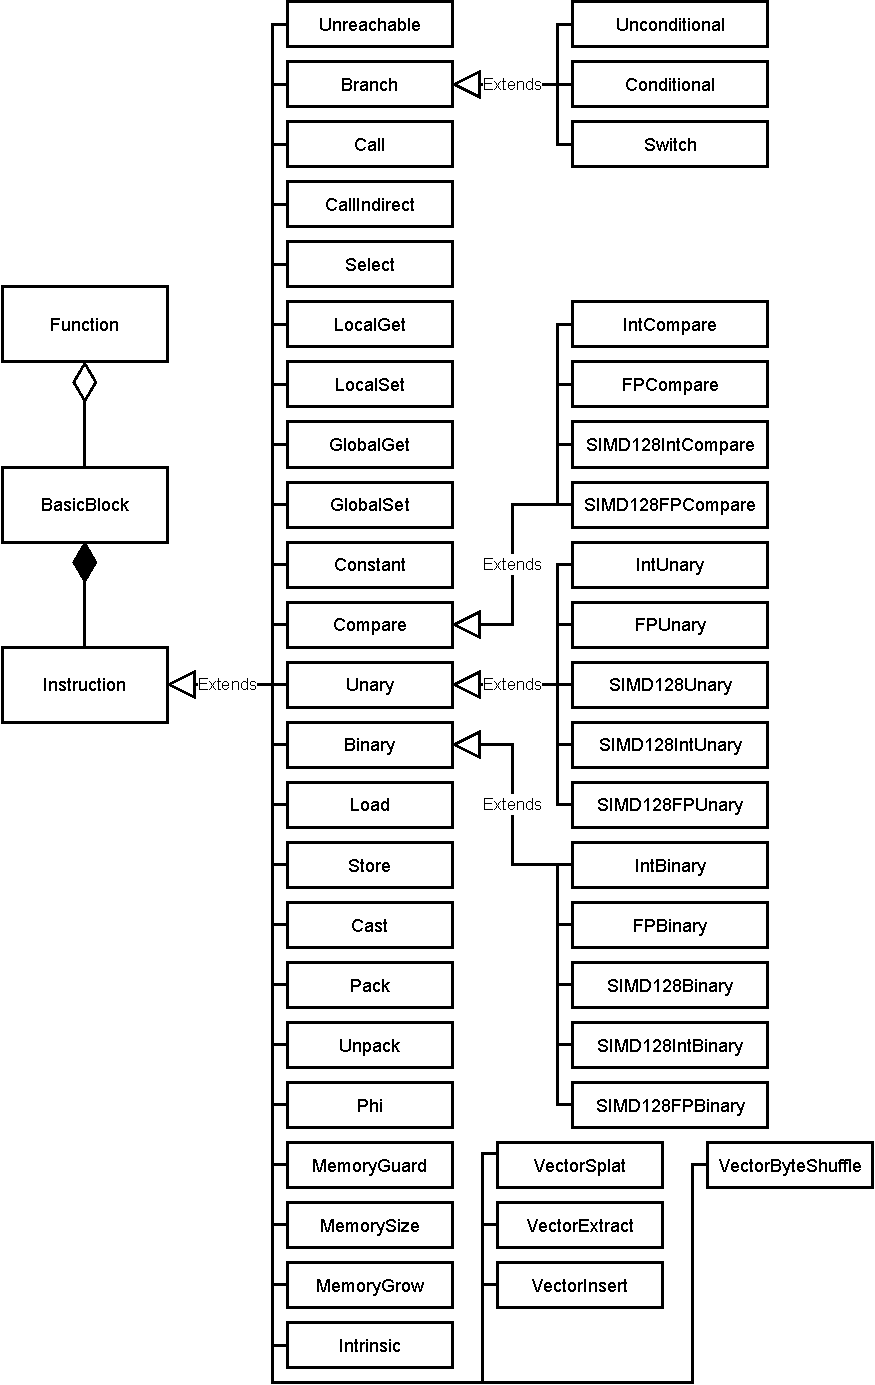
\includegraphics[width=0.8\textwidth]{Images/4.MIR/sablewasm-instruction.pdf}
  \caption{SableWasm MIR Instructions}
  \label{fig:sablewasm-mir-inst}
\end{figure}

\paragraph{Terminating instructions}
As discussed above, SableWasm splits the function control flow into basic
blocks containing the maximum number of consecutive instructions without
control flow transfer. In addition, SableWasm, similar to many other SSA form
instruction sets, defines a particular group of instructions called terminating
instructions. These instructions signal a control flow transfer out of the
current basic block, and they must only appear as the last instruction in any
given basic block. SableWasm defines four different terminating instructions:
unreachable, unconditional branching, conditional branching, and table
branching. If the control flow reaches a \texttt{Unreachable} instruction,
the runtime system will signal a runtime panic. The \texttt{Unreachable}
instruction in SableWasm is identical to its counterpart in WebAssembly in
terms of semantics. The \texttt{Unconditional} instruction is an unconditional
control flow transfer, as the name suggests. It refers to a target basic block
as the operand. At runtime, the instruction will always transfer the control
flow to the target basic block. \texttt{Unconditional} is similar to the
\texttt{br} instruction defined in WebAssembly specification. On the other hand,
\texttt{Conditional} is a conditional branching. It takes a value and two
target basic blocks as its operands. At runtime, the instruction will first
compare the value against integral value zero. If the value equals zero, the
instruction will transfer the control flow to the `false' basic block,
otherwise, to the `true' basic block. SableWasm's \texttt{Conditional}
instruction is similar to \texttt{br.cond} defined in WebAssembly. The last
terminating instruction defined in SableWasm is \texttt{Switch}.
\texttt{Switch} instruction is comparable to the \texttt{br.table} instruction
in WebAssembly. The instruction takes a value, a list of target basic blocks,
and a default branching basic block as its operands. At runtime,
\texttt{Switch} will interpret the value as an integral value and dispatch
accordingly. If the value is within the branching list's range, it will
redirect the control flow to the target basic block referred to by the index.
Otherwise, \texttt{Switch} will transfer the control flow to the default basic
block.

\paragraph{Function call}
In SableWasm, we provide two instructions for function calls defined in
WebAssembly specification: direct function calls and indirect function calls.
\texttt{Call} represents a direct function call where the callee is known at
compile time. It takes a function and a list of arguments as operands. On the
other hand, \texttt{CallIndirect} defines an indirect function call. It
implements the indirect function call protocol described in the WebAssembly
specification. A quick reminder, in WebAssembly, an indirect function call takes
an indirect table, the table index, the expecting function type, and a list of
values as arguments. At runtime, the system should first check if the index is
valid for the indirect table and fetch the function pointer and its actual
signature accordingly. Then, the system should compare the signature against the
expecting type. If the signature matches, the runtime system will
transfer the control flow to the function referred to by the function pointer.
Implementing the signature verification mechanism is backend-specific; we will
return to this topic in the next chapter. Note that we do not treat function
call instructions as terminating instructions, even though they transfer the
control flow to other locations. In SableWasm MIR, we follow the design like
that used in the LLVM intermediate representation, where it is assumed that
the control flow will continue to the next instruction after returning from the
function call. Hence, from the basic block's local perspective, their control
flow is pre-determined, and there is no difference compared to other
non-terminating instructions.

\paragraph{Local and global variable access}
In WebAssembly, instructions have access to locals defined by their parent
functions and global variables defined by their enclosing module. The SableWasm
MIR defines getter and setter instruction for both local and global variables to
implement the specification. Their semantics are the same compare to
WebAssembly's counterparts. We will skip the detail here, but one can consult
the WebAssembly specification for detailed information.

\paragraph{Numerical operations}
In SableWasm, we classify the numerical operations into three different
categories, the \texttt{Compare} instructions, \texttt{Unary} instructions, and
\texttt{Binary} instructions. The \texttt{Compare} instructions implement the
comparison between values, such as `equal to'. They always yield a 32-bit
integer as WebAssembly specification suggests. The \texttt{Unary} and
\texttt{Binary}, as their name suggests, perform unary and binary operations
between values. The result of \texttt{Unary} and \texttt{Binary} instruction is
dependent on the opcode. On the other hand, we can also orthogonally classify
the instructions into integer, floating-point, packed integer, and packed
floating-point numbers. Note that in MVP WebAssembly, there are only integer and
floating-point value operations; the SIMD operation extension proposal adds the
packed value operation to the instruction set. In the WebAssembly SIMD extension
proposal, the vector value does not store its size and content information in
the types. Instead, the packed value instructions' opcodes keep track of the
shape of the vector values, which leads to the bloated instruction opcodes. In
SableWasm, we separate the instruction opcode from the vector shape. For each of
the packed value operations, it must have either a \texttt{SIMD128IntLaneInfo}
or \texttt{SIMD128FPLaneInfo}. Figure~\ref{fig:sablewasm-mir-inst} shows all the
classes of numerical operations defined in SableWasm. For detailed opcodes in
each numerical instruction class, one can consult SableWasm's source code.

\paragraph{Load and Store}
\texttt{Load} and \texttt{Store} instruction provides access to the linear
memory for SableWasm MIR. Although in the current version of WebAssembly, the
module can contain at most one linear memory, and all WebAssembly's load and
store instructions implicitly refer to this linear memory \footnote{This might
  change in the future version of WebAssembly.}. In SableWasm MIR, we take a
different approach. The SableWasm MIR's \texttt{Load} instruction takes a linear
memory and an integer value as operands. At runtime, the value will be treated
as the address (or offset) to the start of the linear memory, and the
instruction yields the fetched result. In WebAssembly, the \texttt{load}
instruction associates with a type and an extension method. For example,
\texttt{i32.load8\_s} loads an 8-bit integer from the linear memory, and then
sign extends the fetched byte into a 32-bit integer. In SableWasm, the
\texttt{Load} instruction associates to a type and an integer value, namely the
load width. The load width must equal to or smaller than the width of the type.
Also, SableWasm \texttt{Load} always perform zero-extension on loaded value.
Hence, when translating WebAssembly's sign-extended load into SableWasm's
\texttt{Load}, one must combine the load instruction with a cast instruction.
We will come back to this in chapter~\ref{chapter:mir-translation-optimization}.
The \texttt{Store} instruction
also associate with a store width. Like the load width defined for \texttt{Load}
instruction, the store width must also be equal to smaller than the store value
type's width. The system will first bit truncate the value at runtime and then
store the result into the linear memory. One may notice that in SableWasm, we
erase the alignment attribute and offset attribute defined in WebAssembly.
Currently, we do not support alignment hints from the WebAssembly module. In
SableWasm, the \texttt{Load} and \texttt{Store} always have the alignment
requirement of one byte. This implies that the \texttt{Load} and \texttt{Store}
can happen anywhere in the linear memory, corresponding to WebAssembly's linear
memory specification.

\paragraph{Linear memory manipulation}
WebAssembly specification defines two instruction that works with linear
memories: \texttt{memory.size}, \texttt{memory.grow}. Like the WebAssembly's
\texttt{load} instruction we covered in the previous paragraph, all these
instructions operate over the implicitly defined unique linear memory within the
module. In SableWasm, we provide similar \texttt{MemoryGrow} and
\texttt{MemorySize} instruction. The semantics of SableWasm's memory
manipulation instructions are the same as their WebAssembly counterparts, except
that the linear memory needs to be explicitly stated. In SableWasm, we introduce
one additional instruction, \texttt{MemoryGuard} which is an explicit memory
boundary check. In WebAssembly, all \texttt{load} and \texttt{store} instruction
need to check for linear memory out of bound error before access. SableWasm
separates the bound check from the memory access. One advantage of this is that
one may implement static memory bounds check elimination optimization over
SableWasm MIR. Additionally, one backend may provide different strategies for
handling boundary checks, such as utilizing invalid virtual memory pages with
the operating system's help. In this case, we only need to modify the
translation pattern for \texttt{MemoryGuard}. \texttt{MemoryGuard} takes a
linear memory and an integer value as the operand. It also associates with an
integer immediate, known as the guard width. At runtime, the system will perform
a boundary check over the linear memory starting from the given address to
determine if it contains at least a given number of bytes ahead. If there are
not enough bytes available, the system should signal a runtime panic.

\paragraph{Pack and Unpack}
WebAssembly multivalue specification \footnote{WebAssembly Multi-value Proposal:
  \url{https://github.com/WebAssembly/multi-value}} relaxes the constrains on
the function type. Functions now can return multiple values instead of at most
one value. To support these features, we introduce \texttt{Pack} and
\texttt{Unpack} instructions, along with extending WebAssembly's type system.
\texttt{Pack} instructions group multiple values into a single ordered tuple,
while the \texttt{Unpack} reverse the operation by retrieving the value from
tuples by index. In the case where a function returns multiple values, we thus
use a tuple instead. SableWasm treats tuples as first-class values; however,
currently, tuples cannot be recursive. We will come back to this
in chapter~\ref{chapter:mir-translation-optimization},
when we visit the type systems of SableWasm MIR. The index of the
\texttt{Unpack} must be an immediate value in the current version of SableWasm
MIR and is verified at compile time.

\paragraph{Vector operations}
In the previous paragraph, we introduce the numeric operations defined in
SableWasm MIR. However, several instructions do not fit into either
\texttt{Unary} or \texttt{Binary} instructions. Hence, to faithfully support the
SIMD operations introduced by the extension proposal, we add four
vector-specific operations into SableWasm MIR. They are \texttt{VectorSplat},
\texttt{VectorExtract}, \texttt{VectorInsert} and \texttt{VectorByteShuffle}.
\texttt{VectorSplat} will broadcast the operand value to all lanes in the result
vector. SableWasm MIR defines vector splat operation for both packed integer
vector and packed floating-point vector. \texttt{VectorExtract} is similar to
the \texttt{extractelement} defined in LLVM intermediate representation. It
takes a vector as the operand and also associates itself with an immediate
integer value. At runtime, the system extracts the value of the given lane and
yields as a result. \texttt{VectorInsert} is similar to \texttt{insertelement}
defined in LLVM. It will replace the vector operand with a given value and
yields the updated vector as a result. Note that in the WebAssembly SIMD
extension proposal, there are more instructions defined that modify the
individual lane value of the vector, such as \texttt{V128Load32Lane} which
loads a 32-bit value into a specific lane within the vector. In this project,
we would like to keep our instruction set simple; hence, these instructions are
reduced into multiple SableWasm MIR instructions. We will come back to this
in chapter~\ref{chapter:mir-translation-optimization}
when we discuss the instruction reduction rules. The last
instruction we introduced is the \texttt{VectorByteShuffle}.
\texttt{VectorByteShuffle} is similar to \texttt{shufflevector} defined in LLVM,
except that it allows rearranging bytes instead of lanes. Currently, the
\texttt{VectorByteShuffle} only operates over an array of immediate integer
values. Compare to the lane shuffle semantics, byte shuffle semantics provides
more precise control over the result value. One can trivially simulate a lane
shuffle with a byte shuffle. The WebAssembly SIMD extension proposal only
defines shuffle for \texttt{i8x16}, which corresponding to the byte shuffle
semantics. However, in the future, if another shape vector supports shuffle
operation, one can generalize the implementation with minimal modification.

\paragraph{Cast}
\texttt{Cast} models the conversion of values to their equivalent form in other
types. In SableWasm MIR, we do not distinguish between value conversion and
value extension. We treat signed and zero extensions as a kind of value
conversion. The \texttt{Cast} instruction takes a single value as the operand,
and it associates itself with a cast opcode. At runtime, it will perform the
conversion according to the opcode, and if the result cannot be accurately
represented in the target type, the system should signal a runtime error.
The cast opcodes are direct implementations of their WebAssembly counterparts,
and we will skip the detail here. One may refer to the WebAssembly specification
for more details.

\paragraph{Intrinsic}
The last SableWasm MIR instruction we are going to cover in this section is the
\texttt{Intrinsic} instructions. Most WebAssembly instructions can be
represented by using the SableWasm MIR instructions, which we covered earlier in
this section. However, there are still several corner cases. For example, the
WebAssembly SIMD extension proposal defines Q-format rounding multiplication, a
type of fix-point multiplication, for packed 16-bit integers. Another example is
the \texttt{swizzle} operation. A \texttt{swizzle} operation is similar to a
shuffle operation, except that it takes another vector as the shuffle indices
vector instead of an array of immediate integer values. These operations are
only defined for a specific vector shape and will introduce unneeded complexity
to the SableWasm MIR if we generalize them to all possible vector shapes. Hence,
here we group these instructions as the \texttt{Intrinsic} instructions. There
is no direct mapping to LLVM instruction for most of them, even with the
intrinsic functions provided by the framework. Hence, the backend is encouraged
to support these instructions with runtime library routines.

In this section, we discussed the design of the SableWasm MIR instruction set,
and in the next chapter, we will move to the translation strategy between
WebAssembly and SableWasm MIR along with the analysis and transformation
framework.

\section{Translating WebAssembly to MIR}

In this section, we will cover the translation between WebAssembly bytecode and
SableWasm MIR. We have covered the design of SableWasm MIR instructions
previously. One may notice that for most of the instructions, especially for the
numerical operations, SableWasm MIR shares the same semantics as WebAssembly.
Hence, the translation rules for these instructions are pretty trivial, and we
will not cover them in detail in this section. Instead, this section will focus
on the translation rules for the structured control flow constructs and
WebAssembly instructions that require reduction during translation.

\subsection{Structured-Control-Flow Construct}

Translating from stack-based IR to register-based IR is not trivial, especially
when non-linear control flow structures appeared. This problem appeared in many
runtime system implementations, such as Numba \cite{numba}, a just-in-time (JIT)
compiler for Python. Usually, one needs some algorithm to recover the control
flow structure from annoying jump instructions. Luckily, in WebAssembly, we can
translate the stack-based bytecode into register-based basic blocks in linear
time, thanks to the structured control flow constructs and their validation
rules defined in WebAssembly. In this section, we will cover the translation
patterns used for WebAssembly's structured-control-flow constructs, namely
\texttt{block}, \texttt{if} and \texttt{loop}.

\begin{figure}
  \centering
  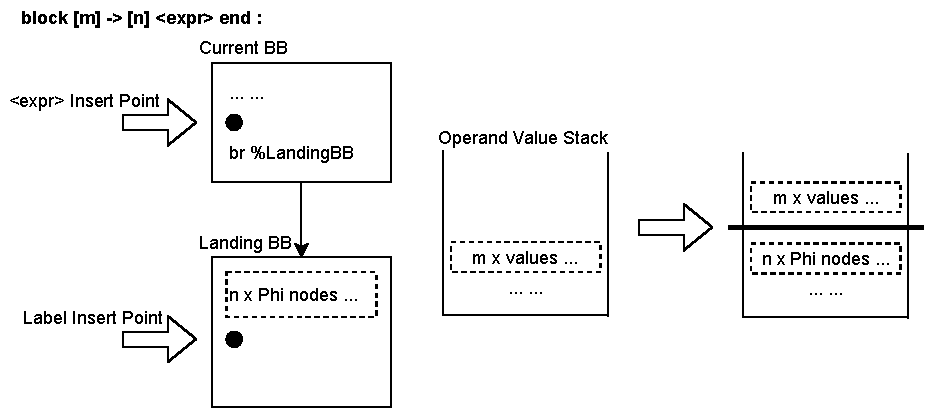
\includegraphics[width=\textwidth]{Images/4.MIR/translate-block.pdf}
  \caption{WebAssembly \texttt{block} translation pattern}
  \label{fig:translate-block}
\end{figure}

\begin{figure}
  \centering
  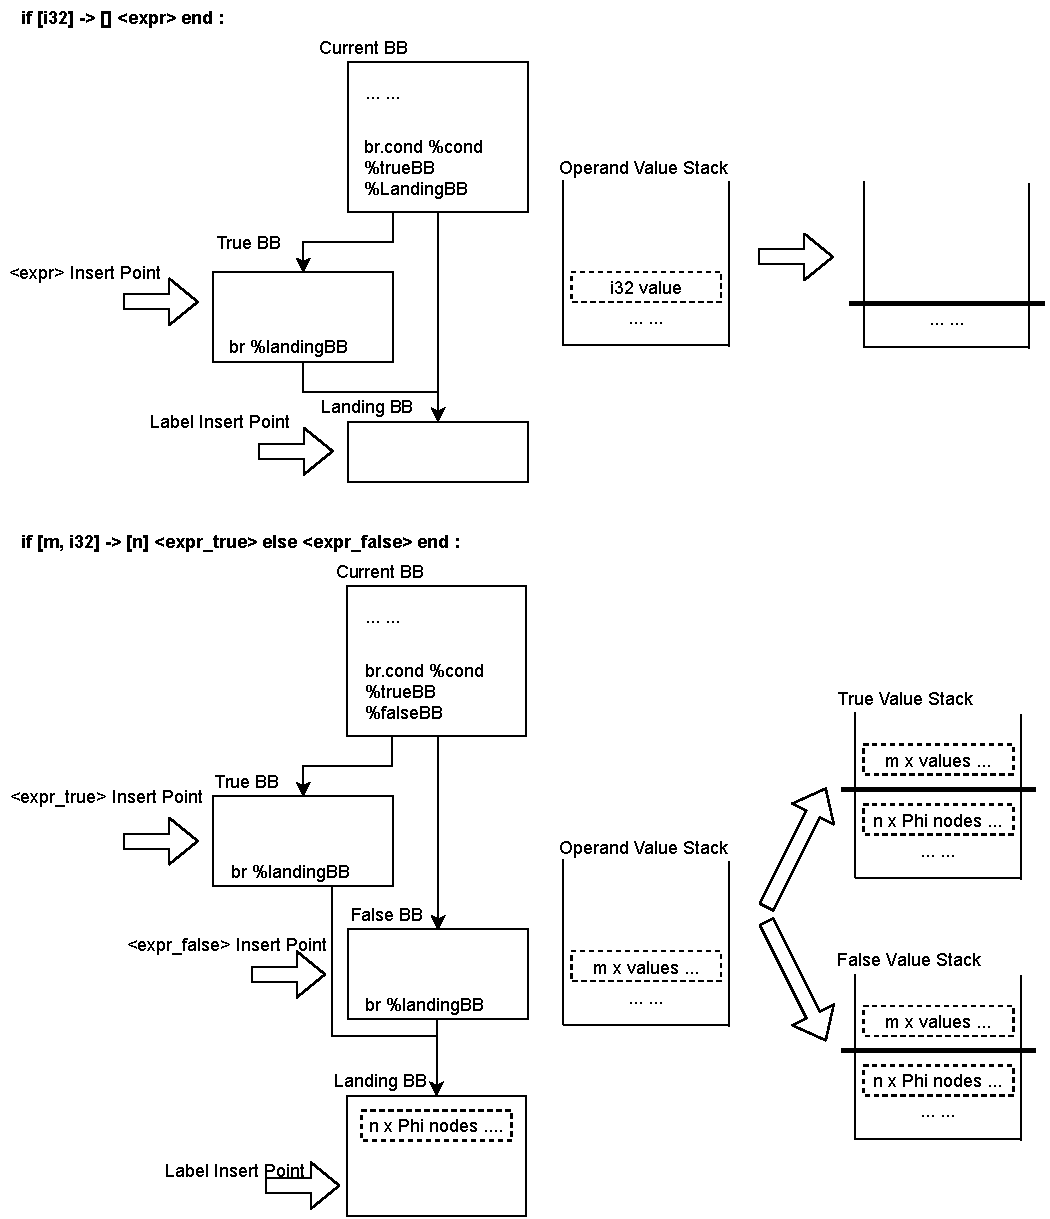
\includegraphics[width=\textwidth]{Images/4.MIR/translate-if.pdf}
  \caption{WebAssembly \texttt{if} translation pattern}
  \label{fig:translate-if}
\end{figure}

\paragraph{Block}
In the background chapter, we provide a general illustration of the three
structured control flow constructs. As a quick recap, \texttt{block} is the
simplest form of a structured control flow construct. It implicitly introduces
a label at the end of its enclosing instructions. A branch instruction
referring to this label will redirect the control flow to the end of the block.
Figure~\ref{fig:translate-block} illustrates the translation pattern for
WebAssembly \texttt{block} in SableWasm MIR. We will first clarify some of the
terminologies we used in the figure, and we will use the same terms later in
the \texttt{loop} and \texttt{if} pattern discussion for consistency.
\emph{Expr Insert Point} refer to the starting position for the generated
instructions when we recursively translate the instructions within the enclosing
expression of the \texttt{block} instruction. Furthermore,
\emph{Label Insert Point} refer to the position for generated instructions when
we finish the recursive translation and resume to the parent expression of the
\texttt{block} instruction. A \emph{label stack entry} is a tuple consisting of
a pointer to the landing basic block, a list of $\phi$ nodes expecting merge
values, and a pointer to the \emph{label insert point}. The translation pattern
for \texttt{block} is pretty simple; we continue on the current basic block and
prepare the landing basic block for the block instruction as a branch
instruction within the expression may refer to the label. Additionally, to fully
support multi-value extension in WebAssembly, we also need to prepare the $\phi$
nodes in the landing basic block. SableWasm generates the $\phi$ nodes based on
the type of the \texttt{block} instruction. WebAssembly validation rules ensure
that the expression within the \texttt{block} can access exactly $m$ values from
the stack and put $n$ values onto the stack. Finally, we will append an
unconditional branch to the landing basic block because in WebAssembly,
if the control flow reaches the bottom of the \texttt{block} expressions, it
will implicitly fall through. For the operand stack, we will first pop $m$
values from the stack as \texttt{block} instruction's type suggests and push the
$\phi$ nodes as the result values. Then, we need to set up the boundary between
the operand stack for the expression contained within the \texttt{block}.
Figure~\ref{fig:translate-block} represents this with the bold line in the
result operand value stack. The last step is to push the $m$ values back to the
stack, as they are passed to the expression within the \texttt{block}.


\paragraph{If}
The next control-flow structure defined WebAssembly is \texttt{if}.
WebAssembly's \texttt{if} is an expression instead of a statement that appears
in many other languages such as C. The \texttt{if} expression can yield some
values indicated by its type. Figure~\ref{fig:translate-if} illustrates the
translation patterns in SableWasm. There are two types of \texttt{if}
instruction defined in WebAssembly specification. The first case is a `partial'
\texttt{if} instruction, where it only contains the `true' branch. From
WebAssembly validation rules, it's easy to show that the only possible type is
\texttt{[i32]->[]}, even with the multi-value extension proposal. This implies
that the expression within the \texttt{if} instruction must start with an empty
operand stack. Hence, the translation pattern for the partial \texttt{if} is
quite straightforward: we only need to pop the condition value from the operand
stack and construct a conditional branch based on this value in the current
basic block. On the other hand, we also have `full' \texttt{if} instructions
with both `true' and `false' expressions. The validation rules ensure that both
expressions must have the same type. The translation pattern is more complex
compare to that of a `partial' \texttt{if}. In this case, we have to prepare the
landing basic block similar to what we did for the \texttt{block} construct.
We need to generate $n$ $\phi$ nodes for data-flow mergers from the `true'
branch, the `false' branch, and any possible branch instruction within both
nested expressions. Similarly, we need to pop $m$ values from the stack for
operand values stack and then push $n$ $\phi$ nodes. And, within both nested
expressions, push $m$ values back to the stack.

\begin{figure}
  \centering
  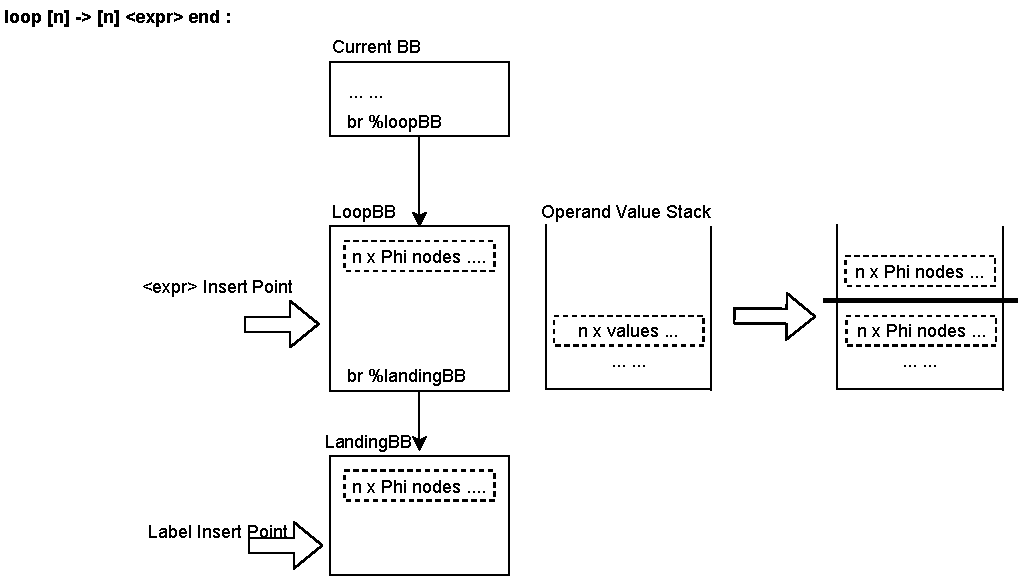
\includegraphics[width=\textwidth]{Images/4.MIR/translate-loop.pdf}
  \caption{WebAssembly \texttt{loop} translation pattern}
  \label{fig:translate-loop}
\end{figure}

\paragraph{Loop}
The last control-flow structure defined in WebAssembly is \texttt{loop}.
Figure~\ref{fig:translate-loop} gives a general illustration of SableWasm's
translation pattern for \texttt{loop} instructions. Similar to the `partial'
\texttt{if} we discussed in the previous paragraph, one can show that, under
WebAssembly's validation rules, the parameter types for the \texttt{loop}
instruction must equal to the result types. The \texttt{loop} instruction is
similar to the \texttt{block} instruction, except that if any branch
instruction refers to it, the branch instruction should transfer the control
flow to the start of the expression within the instruction instead of the end.
Thus, we need to prepare a standalone basic block for the nested expression in
\texttt{loop}, along with the $\phi$ nodes to merge value on each loop
iteration. Note that we also introduce $\phi$ nodes in the landing basic block.
One may argue that there is no need for these $\phi$ nodes, as only one block
can reach the loop exit, and no value merging will occur. Indeed, these
$\phi$ nodes will always be trivial $\phi$ nodes, which have only one
possible value inflow. However, this is due to the limitation of our translation
framework.

In this section, we discussed the translation patterns for WebAssembly
structured control flow constructs. Thanks to WebAssembly validation rules, the
types for these structured control flow instructions explicitly mark value
merging and imply possible $\phi$ nodes. Furthermore, one can show that the
control graph generated above is indeed in SSA form. However, the directly
generated control flow graph is not easily understandable by users. This mainly
comes from two facts. First, the WebAssembly-targeting compiler may generate
awkward patterns to fit in the structured control-flow constructs. Second,
SableWasm translation patterns for structured-control flow constructs are not
optimal.
\subsection{Instruction Reduction}
\label{section:mir-translation-inst-reduction}

This section will cover the instruction reduction rules used when lowering
WebAssembly bytecode to SableWasm MIR. In the background chapter, we mentioned
that one of WebAssembly's design goals is to be as compact as possible. Thus,
when the community designed the WebAssembly instruction set, they fused several
typical instruction sequences into single instructions. For example, SIMD vector
operation extension defines \texttt{v128.load8x8\_s} which first load 8
8-bit integers into a vector, and then sign-extends them into 16-bit
integers. Another example will be \texttt{v128.load32\_lane} which loads a
32-bit value, either a 32-bit integer or a single-precision floating-point
number into a given vector. Such design is understandable for WebAssembly as
binary size does matter when shipping applications over the internet. But, for
SableWasm, a static compiler, we focus more on the size of the instruction set
instead of the size of the intermediate representation. It is harder to write
analysis for a bloated instruction set, as one needs to consider more
instruction cases. Hence, when lowering WebAssembly bytecode to SableWasm MIR,
we replace some WebAssembly instructions with SableWasm MIR instructions
sequences.

\paragraph{Eqz} \quad
\begin{lstlisting}[
    basicstyle=\linespread{1}\small\ttfamily, 
    language=SableWasmMIR, 
    mathescape=true]
[..., %n i32] i32.eqz $\Longrightarrow$ %t0 = i32.const 0; %t1 = int.eq %n %t0
[..., %n i64] i64.eqz $\Longrightarrow$ %t0 = i64.const 0; %t1 = int.eq %n %t0
\end{lstlisting}
WebAssembly defines a unary \texttt{eqz} operations for all integer values. As
the name suggests, \texttt{eqz} compares the operand value against zero and
yields one if true, zero otherwise. In SableWasm MIR, we group all comparison
instructions into the \texttt{Compare} class, and \texttt{eqz} does not fit into
the class as it is not a binary operation. Hence we rewrite the \texttt{eqz} as
\texttt{Compare} instruction with opcode as \texttt{Eq}.

\paragraph{Load} \quad
\begin{lstlisting}[
    basicstyle=\linespread{1}\small\ttfamily, 
    language=SableWasmMIR, 
    mathescape=true]
[..., %base i32] i32.load offset=%offset align=%align $\Longrightarrow$
    %addr = int.add %base %offset
    memory.guard %mem %addr 4
    %t0 = load.32 i32 %mem %addr
[..., %base i32] i32.load16_s offset=%offset align=%align $\Longrightarrow$
    %addr = int.add %base %offset
    memory.guard %mem %addr 2
    %t0 = load.16 i32 %mem %addr
    %t1 = cast i32.extend.16.s %t0
[..., %base i32] i32.load16_u offset=%offset align=%align $\Longrightarrow$
    %addr = int.add %base %offset
    memory.guard %mem %addr 2
    %t0 = load.16 i32 %mem %addr
\end{lstlisting}
In the SableWasm instruction design section, we introduced the \texttt{Load} and
\texttt{MemoryGuard} in SableWasm MIR. A quick recap, SableWasm MIR
\texttt{Load} instruction, compare to its WebAssembly counterpart, assumes
access is in-bound, does not support offset attribute, and always performs
zero-extension on partial loads. Hence, to properly support WebAssembly's
\texttt{load} instructions, we need to reduce them with the strategy shown
above. For load instructions that do not require value extensions, such as
\texttt{i32.load}, we first calculate the actual starting address, perform a
memory boundary check with \texttt{MemoryGuard}, and then perform the memory
read. On the other hand, for a partial load operation, we need first to perform
the load operation using the same protocol as a normal load. Then, if a sign
extension is needed, we will add its corresponding cast instruction. In the
example above, we demonstrate this with WebAssembly's \texttt{i32.load16\_s}.
In this case, SableWasm appends a \texttt{Cast} instruction with opcode
\texttt{i32.extend.16} after the load operation.

\paragraph{Store} \quad
\begin{lstlisting}[
    basicstyle=\linespread{1}\small\ttfamily, 
    language=SableWasmMIR, 
    mathescape=true]
[..., %base i32, %val i64] i64.store offset=%offset align=%align $\Longrightarrow$
    %addr = int.add %base %offset
    memory.guard %mem %addr 8
    store.64 %mem %addr %val
[..., %base i32, %val i64] i64.store16 offset=%offset align=%align $\Longrightarrow$
    %addr = int.add %base %offset
    memory.guard %mem %addr 2
    store.16 %mem %addr %val
\end{lstlisting}
Similar to the \texttt{Load} instruction we discussed earlier, the
\texttt{Store} instruction also assumes the memory access is always in range and
does not provide the offset attribute. However, a \texttt{Store} instruction
will always perform truncation instead of extension. Further, the only possible
truncation is the bit-truncation by discarding bits starting from the most
significant bit. The instruction reduction rules for WebAssembly \texttt{store}
instructions is similar to those for \texttt{load} instructions. In the example
above, we demonstrate the rules with \texttt{i64.store} and its partial store
version, \texttt{i64.store16} which only stores the lowest two bytes into linear
memory. SableWasm inserts \texttt{MemoryGuard} instructions in a similar fashion
to \texttt{load} instructions. Note that we do not insert an explicit
\texttt{Cast} instruction to perform the truncation. A \texttt{Store}
instruction will implicitly truncate the value according to the store width; in
this case, it will truncate the 64-bit integer into a 16-bit integer.

\paragraph{SIMD extension proposal reduction rules} \quad
\begin{lstlisting}[
    basicstyle=\linespread{1}\small\ttfamily, 
    language=SableWasmMIR, 
    mathescape=true]
[..., %lhs v128, %rhs v128] v128.andnot $\Longrightarrow$
    %t0 = v128.not %rhs 
    %t1 = v128.and %lhs %t0
[..., %lhs v128, %rhs v128] i16x8.extmul_low_i8x16_s $\Longrightarrow$
    %t0 = cast i16x8.extend.low.i8x16.s %lhs
    %t1 = cast i16x8.extend.low.i8x16.s %rhs
    %t2 = v128.int.mul i16x8 %t0 %t1
[..., %lhs v128, %rhs v128] i16x8.extmul_low_i8x16_u $\Longrightarrow$
    %t0 = cast i16x8.extend.low.i8x16.u %lhs
    %t1 = cast i16x8.extend.low.i8x16.u %rhs
    %t2 = v128.int.mul i16x8 %t0 %t1
\end{lstlisting}
The SIMD extension proposal introduces approximately 240 instructions into the
WebAssembly instruction set. However, not all of them are simple single
operation instructions. The SIMD extension proposal also follows WebAssembly's
design goal to ensure the compactness of the generated program. The proposal
suggests reduction rules for several SIMD operation instructions, and in
SableWasm, we take advantage of them to reduce the size of the instruction set.
The first applicable instruction is the \texttt{andnot} operation for vectors.
The \texttt{andnot} is equivalent to performing bitwise `not' on the
right-hand-side operand, and then a bitwise `and' operation between the
left-hand-side operand and the temporary result. SableWasm reduces
\texttt{andnot} into a \texttt{not} instruction followed by a \texttt{and}
instruction, as shown in the example above. The second group of reducible
instructions is the \texttt{ExtMul} instructions. The SIMD extension proposal
defines \texttt{ExtMul} for all packed integer vectors except packed 64-bit
integers. They are equivalent to first widening the vector using the appropriate
extension and then multiplying two operands. In the example above, we
demonstrate with \texttt{i16x8.extmul\_low\_i8x16\_s} which performs an
\texttt{ExtMul} operation for packed 8-bit integers. SableWasm implements this
instruction by first performing a sign extension on the lower half of the vector
and multiplying the temporary result as shown above. SableWasm also applies a
similar procedure to \texttt{i16x8.extmul\_low\_i8x16\_u}, except that it uses
a zero-extension in the \texttt{Cast} instruction instead of sign-extension.

\paragraph{SIMD load with zero-padding} \quad
\begin{lstlisting}[
    basicstyle=\linespread{1}\small\ttfamily, 
    language=SableWasmMIR, 
    mathescape=true]
[..., %base i32] v128.load32_zero offset=%offset align=%align $\Longrightarrow$
    %addr = int.add %base %offset
    memory.guard %mem %addr 4
    %t1 = load.32 i32 %mem %addr
    %t2 = const v128 0
    %t3 = v128.int.insert i32x4 0 %t2 %t1
\end{lstlisting}
The WebAssembly SIMD extension proposal also introduces many variations of load
operations. The first variation is the `zero-padding' load operation. The
`zero-padding' load is equivalent to loading a scalar from the linear memory and
then inserting it into a zero-initialized vector. We demonstrate this with the
example above. We first use the protocol we discussed above to load a scalar
32-bit integer. Then, we insert it into a zero vector using
\texttt{VectorInsert} instruction. The WebAssembly SIMD extension proposal
defines `zero-padding' load operations for all packed integers and
packed float-point numbers. The reduction rules for them are similar to the
pattern above.

\paragraph{SIMD load and splat} \quad
\begin{lstlisting}[
    basicstyle=\linespread{1}\small\ttfamily, 
    language=SableWasmMIR, 
    mathescape=true]
[..., %base i32] v128.load32_splat offset=%offset align=%align $\Longrightarrow$
    %addr = int.add %base %offset
    memory.guard %mem %addr 4
    %t1 = load.32 i32 %mem %addr
    %t2 = v128.int.splat i32x4 0 %t1
\end{lstlisting}
The second variation of SIMD vector load is the `load-and-splat' load operation.
This type of load operation is a combination of scalar load operation and vector
splat operation. It first loads a scalar from the linear memory and then
broadcasts the value to all vector lanes. SableWasm uses a similar reduce rule
compared to the `zero-padding' load operation, except that instead of inserting
the scalar into a zero-initialized vector, we use \texttt{VectorSplat} to
broadcast it. The example above demonstrate this with
\texttt{v128.load32\_splat}. Similar to the `zero-padding' load operation,
`load-and-splat' is defined for all packed integers and packed float-point
numbers.

\paragraph{SIMD load lane} \quad
\begin{lstlisting}[
    basicstyle=\linespread{1}\small\ttfamily, 
    language=SableWasmMIR, 
    mathescape=true]
[..., %base i32, %vec v128]
v128.load32_lane offset=%offset align=%align lane=%lane $\Longrightarrow$
    %addr = int.add %base %offset
    memory.guard %mem %addr 4
    %t1 = load.32 i32 %mem %addr
    %t2 = v128.int.insert i32x4 %lane %base %t1
\end{lstlisting}
The next variation of the SIMD vector load operation is the `load-lane' load
operation. The example above demonstrates the procedure with a sample of
WebAssembly's \texttt{v128.load32\_lane} which reads a 32-bit integer from
linear memory and inserts it into a specific lane of a given vector. SableWasm
first lowers the load semantic using the same protocol as we discussed above and
then inserts to the given vector using the \texttt{VectorInsert} instruction.
Again, the WebAssembly SIMD extension proposal defines `load-lane' load
operation for all shapes of packed integers and floating-point numbers. In
WebAssembly SIMD load operation variations, one may already notice that we only
have a width associated with them instead of types. This is because WebAssembly
SIMD operations do not distinguish the shape of the vector. Hence, there is no
difference in loading a 32-bit integer and a single-precision floating number,
as they both consume 32-bit storage. But in SableWasm, we distinguish between
packed integers and packed floating-point numbers for the SIMD instruction shape
record. On the other hand, SableWasm also erases shape information from the
vector value, and it is the responsibility of the instruction to interpret the
value correctly. Thus, when we perform a load operation, we always assume that
we are loading packed integers. In the examples above, the 32-bit load with
translate to `load a 32-bit integer'.

\paragraph{SIMD load and extend} \quad
\begin{lstlisting}[
    basicstyle=\linespread{1}\small\ttfamily, 
    language=SableWasmMIR, 
    mathescape=true]
[..., %base i32] v128.load16x4_s offset=%offset align=%align $\Longrightarrow$
    %addr = int.add %base %offset
    memory.guard %mem %addr 8
    %t1 = load.64 v128 %addr 8
    %t2 = cast i32x4.extend.low.i16x8.s %t1
[..., %base i32] v128.load16x4_u offset=%offset align=%align $\Longrightarrow$
    %addr = int.add %base %offset
    memory.guard %mem %addr 8
    %t1 = load.64 v128 %addr 8
    %t2 = cast i32x4.extend.low.i16x8.u %t1
\end{lstlisting}
The last variation of a load operation is the `load-and-extend' load operation.
It is a combination of partial load and extension on the lower half of
128-bit vectors. In the example above we present examples for
\texttt{v128.load16x4\_s} and \texttt{v128.load16x4\_u}. The previous
instruction loads four 16-bit integers into the lower lanes of the vector and
performs sign-extension on the result to get a packed 32-bit integer vector.
\texttt{v128.load16x4\_u} performs a similar operation, except that it performs
zero-extension instead of sign-extension. A quick reminder, SableWasm MIR
\texttt{Load} instruction can apply to any primitive value type and supports
partial loading by annotating with a smaller load-width. In the case of the
partial load, SableWasm MIR \texttt{Load} always loads bytes starting from the
least significant bit and performs zero-extension on the result. SableWasm takes
advantage of the \texttt{Load} instruction's design when lowering the
`load-and-extend' load operation. In the example above, we partially load a
128-bit vector with a 64-bit value which corresponds to loading four
16-bit integers from the linear memory. Note that this \texttt{Load} instruction
yields a vector of 16-bit integers with four zero values in its higher lanes and
loaded values in its lower lanes. Thus, we only need to perform a \texttt{Cast}
operation with opcode \texttt{i32x4.extend.low.i16x8.s} to reach the desired
result. SableWasm treats \texttt{v128.load16x4\_u} using a similar procedure,
except that it uses zero-extension instead of sign-extension. Finally, like
other load operation variations discussed above, WebAssembly defines the
`load-and-extend' load operation for all packed integer and packed
floating-point numbers.

\paragraph{SIMD store lane} \quad
\begin{lstlisting}[
    basicstyle=\linespread{1}\small\ttfamily, 
    language=SableWasmMIR, 
    mathescape=true]
[..., %base i32, %val v128]
v128.store32_lane offset=%offset align=%align lane=%lane $\Longrightarrow$
    %addr = int.add %base %offset
    memory.guard %mem %addr 4
    %t1 = v128.int.extract i32x4 %val %lane
    store.32 %mem %addr %t1
\end{lstlisting}
Similar to the `load-lane' load operation variation, the WebAssembly SIMD
extension proposal also defines direct lane store instruction for 128-bit
vectors. The above example demonstrates the reduced rules for these
instructions. Let's take \texttt{v128.store32\_lane} as example. SableWasm MIR
first calculates the address and sets up a memory boundary check use a protocol
similar to what we have seen above. Then, it extracts the lane value by using
\texttt{VectorExtract} instruction and stores it into linear memory. Like
WebAssembly \texttt{load} instructions, the \texttt{store} instruction does
not distinguish between packed integers from packed floating-point numbers.
In SableWasm, we always assume the store vector is packed integers.


\section{Analysis Framework}

\begin{figure}
    \centering
    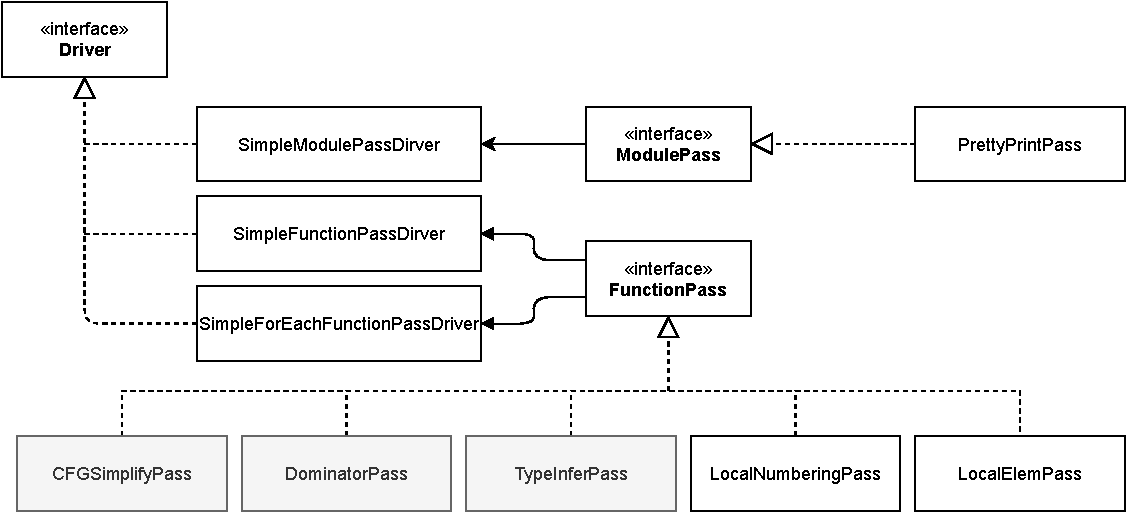
\includegraphics[width=\textwidth]{Images/4.MIR/analysis-framework.pdf}
    \caption{SableWasm MIR Analysis and Optimization Framework}
    \label{fig:sablewasm-mir-analysis-framework}
\end{figure}

SableWasm also implements an analysis and optimization framework over its
middle-level intermediate representation (MIR). The framework consists of two
parts, passes and drivers. The SableWasm analysis and transformation framework
only provides essential support for managing passes, compared to other more
advanced frameworks, such as McSAF\cite{mcsaf}, an optimization framework for
MATLAB language. Figure~\ref{fig:sablewasm-mir-analysis-framework} illustrates
the current state of the framework in SableWasm. Currently, we implement three
different drivers. \texttt{SimpleModulePassDriver} accepts module passes and
operates on the module level. At the time of thesis writing, we haven't explored
inter-procedural analysis for SableWasm MIR in detail, and the only module pass
implemented is the pretty-print pass. In the future, one can add additional
inter-procedural analyses to SableWasm, by implementing the \texttt{ModulePass}
interface. The second driver is the \texttt{SimpleFunctionPassDriver}. As its
name suggests, it manages \texttt{FunctionPass} instead. \texttt{FunctionPass}
implements intra-procedural analysis that operates over basic blocks. SableWasm
currently implements multiple intra-procedural analyses, such as dominator tree
construction and local variable numbering. We will cover these passes in detail
in this section. The last driver in SableWasm is
\texttt{SimpleForEachFunctionPassDriver} which is a wrapper class for
\texttt{SimpleFunctionPassDriver}. It works with \texttt{FunctionPass} but takes
a module as argument.

\subsection{Dominators and Dependence}

Dominator tree and immediate dominance are close related to \emph{static single
    assignment} (SSA) form, and Ron Cytron's classic paper on converting
control flow graph (CFG) to SSA \cite{ibm-ssa} shows that SSA directly derives
from them. The dominator tree represents the dominance relationship between
basic blocks. A basic block is a \emph{dominator} of another if all control flow
reaching the later block must go through the first block. On the other hand,
\emph{immediate dominance} defines a stricter relationship between basic blocks.
A basic block is an immediate dominator of another if it satisfies two
conditions. First, the candidate block must be a dominator block of the second
one. Second, it does not dominate any other blocks that dominate the second
block. Although the SableWasm MIR is already in SSA form, the dominator tree is
still helpful in the later analysis and backend code generation. One may notice
that the dominator relationship in SSA is comparable to the same problem in
graph theory. Indeed, they are the same problem if we treat the basic blocks as
vertices and control flow paths as edges among them.  A direct solution to
compute the dominator set utilizes forward analysis within $O(n^2)$, respecting
to the number of basic blocks in the CFG. More efficient algorithms can yield
the dominator set within almost linear time, such as Tarjan's algorithm
\cite{tarjan-fast-dominator}, and its refined version
\cite{tarjan-fast-dominator-improved}. Currently, SableWasm compiles programs
usually with smaller functions that contain approximately 200 basic blocks at
most. Hence, an efficient complex algorithm does not have too much room for
improvement. In the future, if this becomes the bottleneck of the compilation
pipeline, one should replace the implementation with a better algorithm. This
section will present the forward analysis implementation briefly, and it is a
classic implementation for dominator tree construction.

\paragraph{Formalisms}
In the rest of the section, we will use $dom(\cdot)$ to represent the set of
\emph{strict dominators} for a given basic block. The set of strict dominators
for $A$ is the set of dominators for $A$ subtracting $A$ itself. Hence, block
$A$ is a strict dominator for block $B$ implies that $A \in dom(B)$. Similarly,
$BB_{idom}$ is a immediate dominator for basic block $A$, if and only if,
$(BB_{idom} \in dom(A)) \land (\forall B \in dom(A), BB_{idom} \notin dom(B))$.
Finally, the dominator tree represents all basic blocks with tree nodes and adds
directed edges between them according to the immediate dominator relationship.

\paragraph{Dataflow analysis}
The algorithm is a classic forward dataflow analysis. In this paragraph, we will
quickly cover the key points in the algorithm. For more detailed information,
one should consult Cytron's paper on SSA construction. During pass
initialization, we first set the following,
$\forall A \in BB \setminus \{ BB_{entry} \}, dom(A) = BB$,
where $BB$ denotes the set of all basic blocks that appeared in the control flow
graph, and $BB_{entry}$ denotes the entry basic block for CFG. For the entry
basic block, we set $dom(BB_{entry}) = \{ BB_{entry} \}$ instead. The
initialization value is a conservative guess of the result, and the next step is
to refine it. The iterative step rule is as follow,
$$
    \forall A \in BB, dom(A) =
    \left\{\{ A \} \cup \bigcap_{B \in pred(A)} dom(B)\right\}
$$
Here, $pred(\cdot)$ denotes the predecessor of the given basic block. The
general idea is that for each of the basic blocks, a basic block that dominates
all its predecessors must also dominate the given basic block. The stop criteria
for the dominator analysis are also quite simple. If there are no more changes
in the result, the forward analysis will terminate.

\paragraph{Implementation}
SableWasm implements the forward dataflow analysis we discussed above with class
\texttt{DominatorPass}. In addition, the analysis pass object shares its result
map with a helper class \texttt{DominatorPassResult} which provides helper
methods for accessing the result, such as calculating the immediate dominator
and constructing the dominator tree from the result sets. Finally, SableWasm
uses several techniques to improve the performance, such as modelling the set
with sorted arrays.

In this section, we presented the dominator analysis in SableWasm. The dominator
analysis is quite common among compiler implementations, and it will play a
critical role in the latter part of the project.
\subsection{Control-Flow Graph Simplification}
\label{section:mir-opt-simplify-cfg}

In section~\ref{section:mir-translation}, we illustrated the translation rules
from WebAssembly bytecode to SableWasm MIR. Unfortunately, the translation rules
yield suboptimal control flow graphs. Hence, in this section, we will
incrementally improve the control flow graphs by fixing several obvious issues
we found, such as trivial $\phi$ nodes and unnecessary branching. The control
flow graph simplification also performs \emph{dead code elimination} and
\emph{unreachable basic block elimination}. This section presents the patterns,
along with their transforming strategies used in SableWasm. The general design
of the simplification pass is similar to what one would expect in a peephole
optimizer \cite{peephole-opt}. It iterates through the control flow graph, scans
for matched patterns, and if it finds any optimization opportunities it will
apply transformation strategies immediately. In the future, one may generalize
this simplification pass into a fully-featured peephole optimizer, using a
domain-specific language for patterns similar to Alive
\cite{alive, alive-in-lean} for LLVM to ensure extensibility and correctness of
the patterns. The simplification pass will terminate once the execution reaches
a fixed point, where there are no more optimization opportunities.

\begin{figure}
    \begin{minipage}[t]{.5\textwidth}
        \lstinputlisting[
            basicstyle=\linespread{0.7}\footnotesize\ttfamily,
            language=SableWasmMIR,numbers=left
        ]{Code/4.MIR/simplify-cfg.mir}
    \end{minipage}\hfill
    \begin{minipage}[t]{.5\textwidth}
        \lstinputlisting[
            basicstyle=\linespread{0.7}\footnotesize\ttfamily,
            numbers=left
        ]{Code/4.MIR/simplify-cfg.wat}
    \end{minipage}
    \caption{Control-flow graph simplification example}
    \label{fig:simplify-example}
\end{figure}

\paragraph{Trivial $\phi$ nodes}
The first pattern we found in generated SableWasm MIR is the trivial $\phi$
nodes. Trivial $\phi$ nodes refer to the $\phi$ nodes with only one candidate
value. In section~\ref{section:mir-translation-cfg-construct}, we present the
translation patterns for \texttt{loop}
instructions in WebAssembly and mentioned that the pattern is suboptimal and
will result in trivial $\phi$ nodes. A quick reminder, the \texttt{loop}
instruction needs to insert $\phi$ nodes to the landing basic block, which
necessarily has non-merging control flow as an effect of a limitation in our
translation framework. To address this, we search for
\texttt{\%t0 = phi t [\%t1, \%path]} for all possible type $t$. The
transformation strategy is to replace all appearances of value \texttt{\%t0}
with value \texttt{\%t1}. As the $\phi$ nodes do not map to any operations
and are only introduced by SSA to explicitly mark value merging, removing them
from the control flow graph does not change the semantics of the program. When
replacing the values, SableWasm uses the use-site lists managed by the
\texttt{ASTNode} to boost the performance.

\paragraph{Redundant branching}
The second pattern focus on redundant branching. Redundant branching can also
come from the translation patterns for structured control flow. One may already
notice that we will always generate a landing basic block for the instruction
for every structured control flow construct. However, when the control flow
constructs are the last instructions in their enclosing expression, the landing
basic blocks will only contain a single branching instruction.
Figure~\ref{fig:simplify-example} demonstrates an unoptimized example. On the
right-hand side, the WebAssembly function is a simple function that returns one
when the operand is an even number and zero otherwise. On the left-hand side is
its corresponding SableWasm MIR before simplification. Clearly, \texttt{\%BB:0}
and \texttt{\%BB:1} are redundant. The redundant branch elimination pattern
looks for basic blocks with a single inward flow and attempts to merge them
with their predecessors. In the example, the optimizer will try to merge
\texttt{\%BB:1} and \texttt{\%BB:4} by moving the \texttt{Constant} instruction
into \texttt{\%BB:1}, and redirecting the branching in \texttt{\%BB:1} from
\texttt{\%BB:4} to \texttt{\%exit}.

\paragraph{Dead basic block}
The third pattern we have in SableWasm to simplify the control flow graph is
dead basic block elimination. In figure~\ref{fig:simplify-example}, we have a
dead basic block, namely \texttt{\%BB:2}. These dead basic blocks again come
from SableWasm's translation patterns. When we are translating the control flow
constructs, we always prepare the landing basic block. However, in many cases,
the control flow may not reach the landing basic block. In the example above,
we have a WebAssembly \texttt{return} instruction appear in the \texttt{block}'s
nested expression. The translation patterns for \texttt{return} instruction is
naive, which creates a branch to the exiting block and configures the $\phi$
nodes accordingly. Hence, in this case, the landing basic block will never have
an inward flow. In SableWasm MIR, we do not consider these unreachable basic
blocks malformed. However, in many backends, these are considered bad behaviour.
In addition, these basic blocks also interfere with other optimizations. In the
example in figure~\ref{fig:simplify-example}, \texttt{\%BB:3} does not satisfy
the redundant branching elimination pattern because it does not have a unique
inward flow. However, one of them, \texttt{\%BB:2}, is a dead block. Thus, we
may find more optimization opportunities by removing dead basic blocks from the
control flow graph. In SableWasm, we identify the dead basic block via
a mark-and-sweep algorithm. Starting from the entry block, we mark all the basic
blocks that are reachable. Then we iterate overall basic blocks, and if the
basic block does not have the flag, we add them to the delete list. Finally, we
remove all the basic blocks within the delete list from the control flow graph.

\begin{figure}
    \lstinputlisting[
        basicstyle=\linespread{0.7}\small\ttfamily,
        language=SableWasmMIR,numbers=left
    ]{Code/4.MIR/simplify-cfg-result.mir}
    \caption{Control-flow graph simplification result}
    \label{fig:simplify-result}
\end{figure}

\paragraph{Dead value}
The last pattern we have in the control flow graph simplification pass is dead
value elimination. Dead value elimination is similar to the dead basic block
elimination, except that it works with values instead of basic blocks.
Unfortunately, the example in figure~\ref{fig:simplify-example} does not contain
any dead values. However, the idea is quite simple to understand. Most of the
dead values come from WebAssembly's \texttt{drop} instruction which discards
values from the implicit operand stack. In a non-SSA control flow graph, one
usually needs first to perform \emph{liveness analysis} and \emph{reaching
    definition analysis} to determine if the value is dead. But in SSA, one can
quickly recover this information from the use-definition chain, and in
SableWasm, the base class \texttt{ASTNode} automatically manages it. Thus, the
optimizer will iterate over all values within the control flow graph and check
if others refer to it. If not, it then verifies if the instruction is
\emph{droppable}. A droppable instruction is an instruction such that if we
remove it from the control flow graphs, no observable effects should happen,
similar to the concept of `pure' for functions. Finally, if instructions are
both dead and droppable, the optimizer will remove them from the control flow
graph.

In this section, we covered the flow graph simplification pass in SableWasm. The
optimizer will iteratively run four patterns that we have discussed above until
it reaches a fixed point. Figure~\ref{fig:simplify-result} shows the result of
running these optimizations on the input shown in
figure~\ref{fig:simplify-example}. Compared to the original, the simplified
version is more readable. Moreover, by reducing the number of basic blocks, we
can improve other analyses in SableWasm.

\subsection{Type Inference}
\label{section:mir-opt-type-inference}

This section presents the type system for SableWasm MIR. SableWasm MIR is a
statically typed language with a pretty straightforward type system. However,
one may already notice that SableWasm MIR does not annotate every instruction
with a type, unlike many other compiler intermediate representations. Instead,
SableWasm computes the types for values on-demand via a set of type inference
rules. The type system for SableWasm MIR generalizes from the MVP WebAssembly
type system and its extension proposals with a few modifications. The
formal definition for SableWasm MIR types are as follow,

\begin{lstlisting}[basicstyle=\linespread{1}\ttfamily, mathescape=true]

$\langle$primitive_type$\rangle$ ::= i32 | i64 | f32 | f64 | v128
$\langle$tuple_type$\rangle$     ::= (N, $\langle$primitive_type$\rangle$$\dots$)
$\langle$type$\rangle$           ::= $\langle$primitive_type$\rangle$ | $\langle$tuple_type$\rangle$ | () | $\bot$

\end{lstlisting}

Here we will skip the discussion for \emph{primitive type} and the type checking
rules for its corresponding instructions as they are equivalent to the MVP
WebAssembly type system. The \emph{tuple type} consists of an unsigned integer
and a list of primitive types. They model the return types of multi-value return
functions or \texttt{Pack} instructions. Finally, we introduce the unit type,
$()$, and the bottom type, $\bot$. One can consider the unit type as
\texttt{void} in the C programming language. It represents no value present,
but the type is valid. On the other hand, the bottom type, $\bot$, signals that
the pass cannot assign any valid type to the term. In the rest of this section,
we will focus our discussion on extensions made due to two major WebAssembly
extension proposals, multi-value and SIMD operation.

\paragraph{Multi-value}
WebAssembly multi-value extensions allow functions to have more than one return
values, which is quite interesting. Usually, low-level bytecode representation
does not directly support this feature, and it usually only appears in
higher-level language designs, such as Python. In
section~\ref{section:mir-design-insts}, we introduced
two instructions \texttt{Pack} and \texttt{Unpack}, along with how we represent
multi-value for functions. As a quick recap, SableWasm uses tuples to denote the
multi-value return for functions. The \texttt{Pack} instruction collects values
and constructs a tuple containing them, while on the other hand, the
\texttt{Unpack} extracts primitive values from tuples. Let's focus on the
\texttt{Pack} instruction first. The typing rule for \texttt{Pack} is
straightforward. If we can infer types for all candidate values, we say that the
\texttt{Unpack} instruction has a tuple type consisting of the number of
candidate values and a list of element types. On the other hand, if any of the
candidate values result in a non-primitive type, the \texttt{Pack} instruction
is the $\bot$ type. More formally,
$$
    \frac
    {\Gamma \vdash v_0 \Rightarrow t_0, \dots, v_n \Rightarrow t_n \qquad \forall i, t_i \in primitives}
    {\Gamma \vdash \text{\textbf{pack} } v_0, \dots, v_n \Rightarrow \langle n, t_0 \dots t_n \rangle}
    \qquad
    \frac
    {\Gamma \vdash \exists i, v_t \notin primitives}
    {\Gamma \vdash \text{\textbf{pack} } v_0, \dots, v_n \Rightarrow \bot}
$$
Here the set $primitives$ is the set of all possible primitive types in the
SableWasm MIR type system. For \texttt{Unpack} instructions, the type checker
will first check if the immediate index is within the tuple size. If the index
is out of bounds, the type checker will assign the instruction with bottom type
$\bot$. Otherwise, it will take the type from the tuple specified by the index.
Formally,
$$
    \frac
    {\Gamma \vdash v \Rightarrow \langle n, t_0 \dots t_n \rangle \qquad 0 \leq k \leq n}
    {\Gamma \vdash \text{\textbf{unpack } k v} \Rightarrow t_k}
    \qquad
    \frac
    {\Gamma \vdash v \Rightarrow \langle n, t_0 \dots t_n \rangle \qquad \text{otherwise}}
    {\Gamma \vdash \text{\textbf{unpack } k v} \Rightarrow \bot}
$$
We also generalize the function type in WebAssembly so that SableWasm MIR's
function type will always have a single return value. We use the following
strategy to map WebAssembly's function type into SableWasm MIR function type.
In the case where there are no return values, we translate the return type into
unit type. For example, SableWasm translate \texttt{[i32] -> []} into
\texttt{[i32] -> ()}. On the other hand, if the function type has exactly one
return value, the translation rule is trivial. Finally, when there are multiple
return values, we pack them into a single tuple. For example, SableWasm use
\texttt{[i32] -> (2, i32, f32)} to represent \texttt{[i32] -> [i32, f32]} in
WebAssembly.

\paragraph{SIMD operations}
Section~\ref{section:mir-design-insts} presented the instruction design in
SableWasm MIR. We mentioned
that WebAssembly's 128-bit vector value, added by the SIMD operation extension
proposal, does not store their shape information in the type. WebAssembly's
design gives us two choices in SableWasm when designing a type system for vector
operations. First, we can erase all the shape information for values and
carefully plan the instruction semantics to ensure that all the operations
have defined behaviour at runtime. Second, another approach is to add shape
information back to the values' types. If there is a mismatch in shape
information, either the translation visitor can insert a bit cast, or the type
checker can reject the program. In SableWasm MIR, we take the first approach by
erasing all the shape information from the vector values.
Chapter~\ref{chapter:backend-and-runtime} will introduce the second approach in
detail. The semantics for SIMD instructions in SableWasm MIR follows the
WebAssembly's specification. We always store the value using the little-endian
method and the vectors start their first lane from the least significant bit.

In this section, we talked about the type inference pass in SableWasm MIR.
Similar to the dominator analysis we seen in
section~\ref{section:mir-opt-dominator}, the type infer pass
does not optimize the control flow graph. But they are critical in the backend
when we lower the SableWasm MIR into LLVM. We will come back to this in detail
in chapter~\ref{chapter:backend-and-runtime}.
\subsection{Redundant Local Variable Elimination}

In this section, we are focusing on another common problem that appeared in translated WebAssembly programs. From the WebAssembly validation rule, one may notice that, in MVP, there is no way for instructions in a \texttt{block}, \texttt{if}, or \texttt{loop} to access values beyond their scope. MVP WebAssembly adopts this rule to simplify the validation rules and ensure the safety of the generated module. However, this leads to poor performance in generated code. The WebAssembly compiler needs to push them to the local pool first, and later load them from the pool to push values into the nested expression within the structured control-flow constructs. A non-optimized runtime implementation might emit a store operation to stack memory and a load operation to stack memory. Figure~\ref{fig:redundant-local-elem} demonstrate this problem with an concrete example. The code is selected from a two-dimensional matrix multiplication benchmark test in C programming language and compiled to WebAssembly with WASI enabled Clang compiler \footnote{WASI SDK: \url{https://github.com/WebAssembly/wasi-sdk}}. Here we turn off the multivalue extension to give a better understanding of the problem. The function implements the memory copy procedure, \texttt{memcpy}, that appears in the standard C library. Here we only present a small snippet of the entire function as the original function contains more than 600 instructions and does not fit the thesis length. But, the problem appears in numerous locations in the entire generated control-flow graph. Line 13 and line 18 in figure~\ref{fig:redundant-local-elem} contain a pair of redundant local variable load and store instructions. So, why do we have these redundant load and store instructions here? One may notice that \texttt{\%BB:2} is the condition block that generated in the translation pattern for \texttt{if} instruction, and \texttt{\%BB:3} is the false block for that \texttt{if} instruction. As in MVP WebAssembly, the only possible type for \texttt{if} instruction is \texttt{[i32] -> []}, which consume exactly only one value as condition from the operand stack. Hence, the additional value needs to be awkwardly pass through via the local pool, in this case, value \texttt{\%23}. A better control flow graph should eliminate this \texttt{LocalGet} instruction in line 18 by replacing with \texttt{\%23}, and even better the \texttt{LocalSet} at line \texttt{\%13} if there are no value depends on this store operation.

\begin{figure}
    \lstinputlisting[
        basicstyle=\linespread{1}\small\ttfamily,
        language=SableWasmMIR,numbers=left
    ]{Code/4.MIR/memcpy.mir}
    \caption{Redundant local variable elimination example}
    \label{fig:redundant-local-elem}
\end{figure}

To address these problems, we implement the redundant local elimination that derived from the point-to analysis\cite{alias-sable, point-to-microsoft, point-to-survey}. The accurate full-scale point-to analysis is hard. In fact, the problem is undecidable \cite{point-to-undecidable}. Compared to the full-scale point to analysis, the SableWasm MIR redundant local variable elimination is relatively simple. First, we only have one layer of indirection. In a full-scale alias analysis, one might need to construct a graph to get the whole picture. In SableWasm's redundant local elimination analysis, we only have one layer of indirection, a value referring to a local variable. Second, there are no complex data construct in WebAssembly. Finally, one complicated problem in alias analysis is around \texttt{Call} instructions. In a full-scale point-to analysis, one needs to utilize inter-procedural analysis to compute the result accurately. However, in SableWasm MIR, the local variable is private to its enclosing function, and the local alias can only happen within the function. Thus, when performing the local variable alias analysis, we can safely assume the calls do not affect the result. The redundant local variable elimination analysis splits into three parts, local variable aliasing, local get elimination and local set elimination.

\paragraph{Local variable aliasing}
Local variable aliasing analysis is the first part of the redundant local variable elimination analysis, and it is a forward data-flow analysis. It computes the relationship between local variables and values. We will first go through the result representations in the analysis. We record the possible alias using pairs $\langle \%local, \%value \rangle$, indicating that $\%local$ may contain value of $\%value$. Additionally, we introduce a special value $\%zero$, referring to the implicit zero-initializer at the beginning of the function. The initialization for `In' sets is straightforward. We initialize its `In' set with all locals implicit initialized to zero for the entry block and empty for any other basic blocks. Initially,  any basic block except the entry block has no information on local variable aliasing, and later in the analysis, we will incrementally collect them. The formal definition for `In' sets initialization is as follows. Here we use $locals$ to denote all local variables defined in the function, and $BB_{entry}$ refers to the entry block.
\begin{align*}
    IN(BB_{entry}) & = \{ \langle x, \%zero \rangle : x \in locals \} &                                 \\
    IN(BB)         & = \{ \}                                          & \forall BB . BB \neq BB_{entry}
\end{align*}
Next is the merge operator for the analysis. The merge operation for the local variable aliasing is a simple union operator, as the data flow may come from any predecessor blocks. The last part of the analysis is the `Gen' set and `Kill' set for instructions. In local aliasing analysis, we only need to consider for \texttt{LocalSet} instructions as they are the only instructions that create a point-to relationship between local variables and values. For clarity, let's assume the \texttt{LocalSet} instruction is \texttt{local.set \%local \%value} which set the local variable $local$ with $value$. The `Gen' set for the instruction is quite straightforward, and it is $\langle local, value \rangle$. The `Kill' set is more interesting. It is the set of pairs that has local variable $local$ because, after a \texttt{LocalSet} instruction, any point-to relationships for this local variable are outdated. More formally,
\begin{align*}
    \bowtie(BB)                                   & =
    \bigcup_{pred \in Pred(BB)} OUT(BB)               \\
    GEN(\text{\textbf{local.set} } local\ value)  & =
    \{ \langle local, value \rangle\}                 \\
    KILL(\text{\textbf{local.set} } local\ value) & =
    \{ \langle local, v \rangle : \forall v \in values \}
\end{align*}
Here we use $values$ to denote the set of all available values within the control-flow graph. The stop criteria for the analysis are simple. If there are no more changes in the result sets, the local variable aliasing analysis will terminate. It's easy to show that the process will eventually complete. The size of all results sets is non-decreasing between iterations, and there is an upper bound for the set cardinality. In this paragraph, we present the local variable aliasing analysis we used in SableWasm MIR. It is closely related to the existing point-to analysis and aliasing analysis.

\paragraph{Local variable get elimination}
After we compute the relationship between local variables and the values, we can then start performing local variable eliminations. Here, we begin by iterating through all instructions, and for \texttt{LocalGet} instructions, we exam the local variable aliasing results at that point. If the aliasing is unique, we can proceed to the next step of elimination; otherwise, we will leave the \texttt{LocalGet} unchanged. If the aliasing refers to $\%zero$, we will replace the \texttt{LocalGet} instructions with a \texttt{Constant} instructions with zero value. On the other hand, if the aliasing refers to a unique value, we will replace any occurrence of \texttt{LocalGet}'s value with it. Note that this replacement does not violate the SSA form of the control-flow graph. Assume there is an instruction that refers to the value yield by \texttt{LocalGet}, then its enclosing basic block is either dominated by the \texttt{LocalGet}'s block, or that instruction is a Phi node. One may show that the unique point-to value must dominate the \texttt{LocalGet}'s block; otherwise, the local variable refers to more than one value. Thus, if we replace a dominating value with another dominating value, the SSA constraints still hold.

\paragraph{Local variable set and local variable elimination}
The last part of the analysis is the local variable set and local variable elimination. Once we finished the local variable get elimination, we can reduce these problems into dead-code elimination. SableWasm MIR consider a \texttt{LocalSet} instruction dead if the local variables has no \texttt{LocalGet} refers to it. One may notice that this problem is isomorphic to liveness analysis. Indeed, in SableWasm MIR, we perform a liveness analysis on local variables to determine which local variables are still alive based on the \texttt{LocalGet} instructions and perform dead \texttt{LocalSet} elimination based on the result. We will skip the details on liveness analysis here as they are quite standard in compiler implementations. One could consult the paper\cite{fast-liveness} for more details. Finally, we can perform dead local variable elimination. Compare to dead \texttt{LocalSet} elimination, removing redundant local variable is quite straightforward. We only need to iterate through the use-site list to check if there exists any reference to the local variable; if not, we remove the instruction from the function.